% Two-column conference layout (acmart sigconf, same as paper4_when_not_rewrite
% and paper1_knc_net_2col). DERIVED from paper3_lexicon.tex (elsarticle
% preprint = archival version) with conference-length trims: §2/§5/§6.3/§6.4/§8
% compressed; §6.5 isolated experiment and §7 monitors kept in full.
% Target venue: JCDL (double-blind → anonymous).
\documentclass[sigconf,nonacm,anonymous]{acmart}
\usepackage{booktabs}
\usepackage{tabularx}
\usepackage{multirow}
\usepackage{graphicx}
\usepackage{xeCJK}
\setCJKmainfont{Noto Serif CJK SC}
\emergencystretch=3em
\renewcommand{\dbltopfraction}{0.92}
\renewcommand{\textfraction}{0.06}
\renewcommand{\dblfloatpagefraction}{0.8}
\setcounter{dbltopnumber}{3}
\setcounter{topnumber}{2}
\setcounter{totalnumber}{4}

\begin{document}

\title{When Schema Lexicons Fail: Diagnosing and Repairing Entity-Layer
Collapse in a Production Knowledge Base}

\begin{abstract}
In dictionary-driven entity enrichment, the schema lexicon \emph{is} the
extraction model. We report a production incident in which a category-word
lexicon silently collapsed the entity layer of a 61{,}137-document scholarly
knowledge base: 575 type-level entities (``method'', ``energy'') carrying
${\sim}$19.2M links while every job-level monitor stayed green. We diagnose
the failure across three layers (extraction mechanism, lexicon provenance,
monitoring blindness), repair it with a three-source corpus-presence-attested
lexicon (3{,}702 terms), rebuild the entity layer under production load, and
derive scale-invariant quality monitors. An isolated fixed-code,
fixed-corpus experiment that varies \emph{only the lexicon} reproduces the
collapse signature alone (77 entities, top-10 concentration 0.557, 1.8
concepts/document) and isolates the repair effect (493 entities, 0.316,
3.7); the rebuilt layer carries 1{,}871 entities, 25.1M links, and a
functioning relation layer; distinct concepts per document rise
15.7$\to$37.8 with document coverage 48.5\%$\to$98.5\%; an LLM-assisted
audit puts link precision at 0.85 (95\% CI [0.77, 0.91]; 1.00 on domain
terms, n=25). The generic tail survives repair (9\% of links sit on the
single ambiguous symbol ``be''), retrieval-facing gains are not
attributable to the lexicon alone (entity-channel ablation bitwise null),
audit is model-assisted rather than human-adjudicated, and monitor
thresholds are post-hoc on 13 libraries --- limitations stated up front.
\end{abstract}

\keywords{knowledge base construction \and schema quality \and terminology
extraction \and entity linking \and production incident \and observability}

\maketitle

\section{Introduction}\label{sec:intro}

Scholarly knowledge platforms increasingly generate subject schemas with
LLM assistance: a batch tool drafts entity types with a handful of aliases
each, a validator checks structural well-formedness, and the schema is
bound to knowledge bases as configuration~\cite{llmonto}. When the
enrichment pipeline then extracts mentions by \emph{dictionary scan}, the
schema's alias list becomes the extraction surface --- the lexicon is not
descriptive metadata but operative infrastructure.

The failure we report: a 61{,}137-document nuclear-electronics knowledge
base accumulated ${\sim}$19.2M entity links onto \textbf{575 canonical
entities}, every one a bare type word (``method'', ``parameter'',
``energy''); a 13{,}408-document physics library showed the same disease
at 2{,}018 entities. Every operational signal stayed green --- jobs done,
throughput nominal, link volume reading as growth. The graph had
degenerated into a bipartite type--document index that was row-level
indistinguishable from a populated knowledge graph.

We contribute: (1)~a forensic record of schema-lexicon-induced entity
collapse, with the timeline and the observables that expose it (top-10
link concentration and the top-entity name audit; cardinality only
corroborates); (2)~a three-source corpus-presence-attested lexicon
construction method (seed transplant, corpus-candidate classification,
bounded expansion) that repaired both schemas without manual
lexicography; (3)~an \emph{isolated} fixed-code fixed-corpus experiment
showing the lexicon variable alone reproduces the collapse and its
repair; (4)~a full-chain production rebuild whose forensics corrected our
own incident log (an \texttt{INSERT IGNORE} mis-attribution mechanism and
a seven-hour ``zero growth'' claim contradicted by row timestamps); and
(5)~four gold-free quality monitors with a 13-library calibration.

\section{Background and Prior Art}\label{sec:related}

Dictionary- or gazetteer-driven entity recognition is one of the oldest
NER traditions~\cite{nerSurvey}; corpus-statistical term recognition
goes back to C-value/NC-value~\cite{cvalue} --- our corpus-candidate
source is that program reborn with an LLM classifier. Knowledge-graph
refinement~\cite{paulheim} and production data validation~\cite{tdd}
address adjacent problems. What prior art does not cover is the specific
failure locus: when the dictionary \emph{is} the extraction model, a
structurally valid but terminologically hollow schema passes every
existing gate.

Our pipeline extracts mentions in stage K1 by normalized dictionary scan
(CJK substring; ASCII word-boundary with optional plural, case-folded);
K2 links mentions to canonical entities by normalized form + type; K3
adjudicates typed relations with an LLM; K4 projects to the graph store.
The healthy reference case in the same deployment --- hydrogeology, 78
documents, a hand-evolved 3{,}742-term lexicon, 1{,}608 entities ---
establishes plausibility, not causation: domain, scale, and provenance
all differ.

\section{The Collapse, Forensically}\label{sec:collapse}

\textbf{Observation} (Table~\ref{tab:collapse}). During an unrelated
storage investigation (2026-10-08), a routine entity-quality sample
returned type words where domain concepts were expected.

\begin{table}[t]
\centering
\caption{The collapse, measured, with snapshot provenance (``bckp.'' =
2026-10-06 cold backup, mid-enrichment; ``disc.'' = discovery-day).}
\label{tab:collapse}
\small
\begin{tabularx}{\columnwidth}{@{}lXX@{}}
\toprule
KB & Entities & Links \\
\midrule
nuclear (61{,}137 docs) & \textbf{575} (disc.) / 503 (bckp.) & \textbf{${\sim}$19.2M} (disc.) / 4.81M (bckp.) \\
physics (13{,}408 docs) & \textbf{2{,}018} & 2.23M (bckp.) \\
hydro (ref., 78 docs) & 1{,}608 & 719{,}515 \\
\bottomrule
\end{tabularx}
\end{table}

\textbf{Mechanism.} When the alias set for type \emph{method} contains
common words, every occurrence in 7.2M chunks becomes a mention, and K2
folds them onto one entity per (form, type). The mechanism executed
faithfully on degenerate input; the dictionaries were the schemas ---
the batch generator produced a category taxonomy where a terminology was
needed~\cite{iso1087}.

\textbf{Timeline} (compressed): 10-08 discovery $\to$ root cause,
lexicon tool built/run/committed, teardown $+$ 766{,}501-event
re-enqueue; 10-08 night: silent mis-attribution window (below); 10-09
drain completes, statistics recomputed, two smaller diseased libraries
treated; 10-09/10: retrospective audits (scoped refresh, channel
ablation, link audit, fleet-wide concentration) and manuscript. The
compression is real; the evaluation is retrospective, not
pre-registered.

\textbf{Why nothing fired.} Job-level observability was all green; link
volume read as success. The observables that expose the collapse are the
concentration of links on the top entities (collapsed: 0.419, measured
from the pre-incident backup, versus 0.18 for the reference case) and
the name distribution of those entities (pure type vocabulary). Entity
cardinality per document --- a factor of 2{,}192 below the reference
case (0.0094 vs 20.6) --- corroborates, but is gameable in both
directions, so it is the secondary signal.

\section{Corpus-Attested Lexicon Construction}\label{sec:lexicon}

Three sources, all gated by corpus presence (a term the corpus never
attests is not admitted --- presence is necessary, not sufficient, for
termhood): \textbf{seed transplant} (2{,}284 terms from a healthy
near-domain library); \textbf{corpus-candidate classification} (top
8{,}000 unigram/bigram n-grams by chunk frequency over a
3{,}000-chunk-per-KB sample, frequency $\geq$5 after boilerplate and
stop-word filtering; an LLM classifies each into a schema type or
rejects it); \textbf{per-type expansion} ($\leq$60 per type). Catch-all
types accept no classified noise; cross-type conflicts resolve by
specificity. Classifier: Qwen3.6-35B-A3B (AWQ 4-bit, community build;
served under a historical alias), temperature 0.2, single idempotent
run. Output: nuclear v2.1 = 3{,}702 terms; physics v1.1 = 1{,}279.

\section{Rebuild at Scale --- and a Corrected Incident Log}\label{sec:rebuild}

Per knowledge base: delete graph vertices with edges, the four
relational tables in bounded chunks, and the search-side projection;
re-enqueue all documents through four stages. The printed
``766{,}501 jobs'' counts \emph{events}, not distinct doc-stages
(74{,}545$\times$4 = 298{,}180): the surplus is the repair window's
re-enqueue waves (silent-empty reset 75{,}831; zero-effect
relations/graph resets ${\approx}$149k; watchdog-deletion recovery
${\approx}$122k; small libraries 5{,}772).

Four pipeline pathologies surfaced and were fixed (committed, measured):
an unbounded projection join that saturated a 112-core database at load
500 (scoped to per-document mentions: 25+ min $\to$ seconds); two
link-insertion deadlock classes (deadlock 1213 $\to$ 0); and an
$O(N^2)$ alias check the richer lexicon itself amplified (101\,s
$\to$ 0.05\,s per task; fleet link throughput 8/min $\to$
1{,}100/min --- a window-level aggregate, with the cache's isolated
contribution measured at task level).

\textbf{The fifth pathology, revisited.} Our log recorded a
parameter-order bug in a single-statement link writer whose rows
\texttt{INSERT IGNORE} ``silently swallowed'' for seven hours. A minimal
reproduction on the production engine (MySQL 8.4,
\texttt{STRICT\_TRANS\_TABLES}, faithful DDL) sharpens the mechanism:
the NULL from \texttt{UNHEX('alloy')} is \textbf{replaced by the
implicit default 0x00$\times$16 and the row is inserted} --- into a
ghost bucket invisible to every per-KB query --- and a later correct
re-insert for the same (mention, entity) pair is \textbf{silently
skipped by the unique key}: the orphan poisons the repair unless
deleted first (production carries zero 0x00 rows today, so cleanup
happened). The duration claim also fails row-level forensics: the
registry's own \texttt{created\_at} histogram (Figure~\ref{fig:telemetry})
shows KB1 inserting at 1.0--2.3M rows/hour \emph{through} the nominal
silent window and KB2's entire link layer landing in one hour. We keep
the log entry and its correction side by side: incident narratives
written from job dashboards are themselves unverified claims.

\begin{figure}[t]
\centering
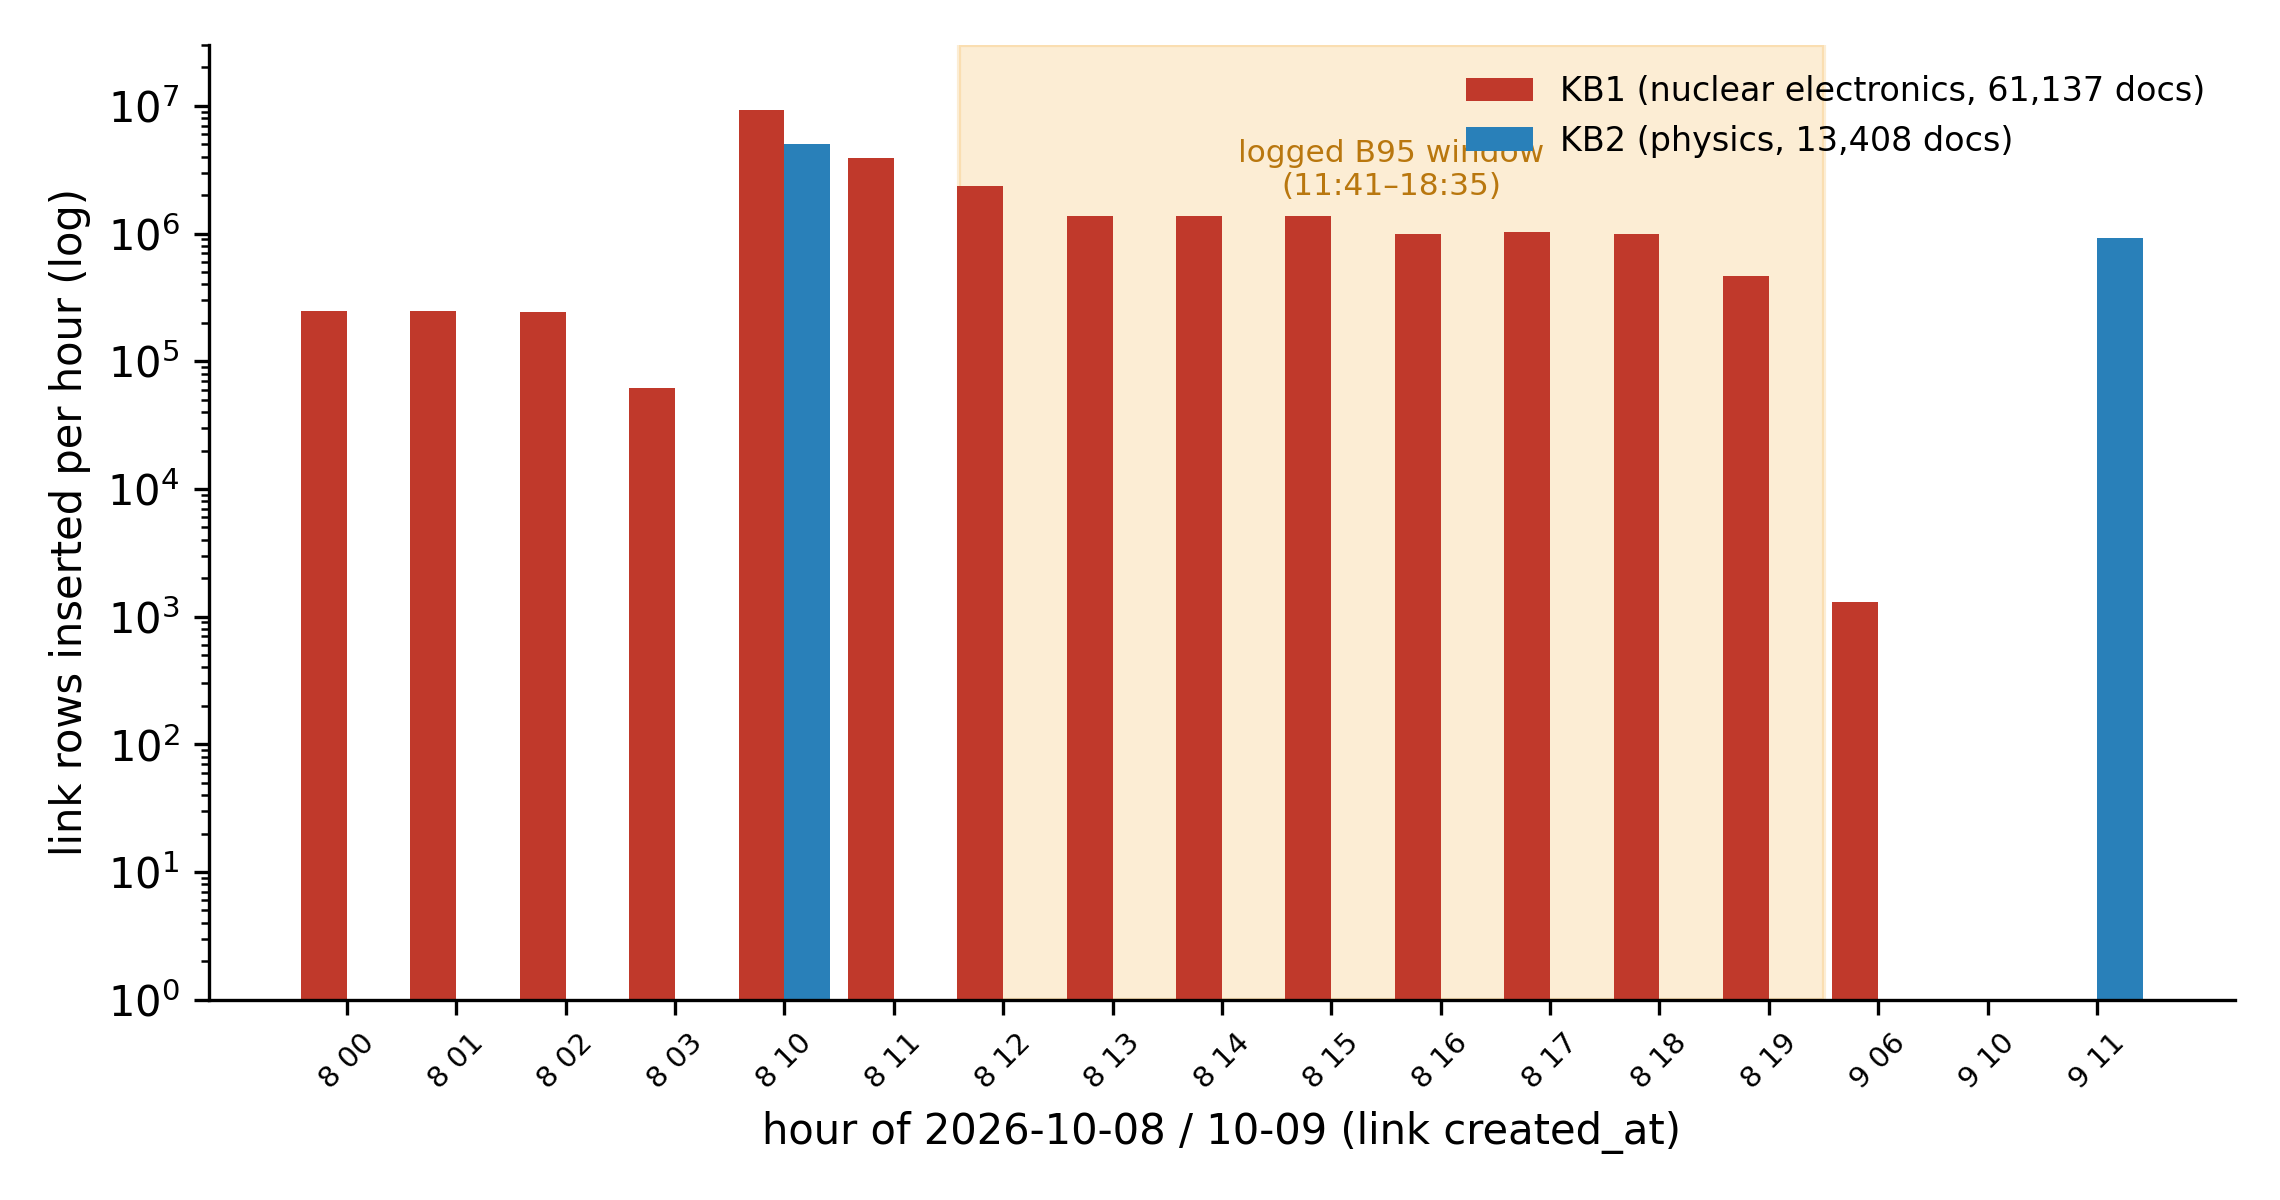
\includegraphics[width=\columnwidth]{figs/fig_rebuild_telemetry.png}
\caption{Rebuild telemetry from the link registry's own timestamps. The
shaded band is the \emph{logged} silent window; inserts continue
through it --- the timestamp correction of \S\ref{sec:rebuild}.}
\label{fig:telemetry}
\end{figure}

\section{Before/After}\label{sec:after}

\begin{table}[t]
\centering
\caption{Entity layer before/after, with snapshot provenance.}
\label{tab:after}
\small
\begin{tabularx}{\columnwidth}{@{}lXX@{}}
\toprule
Metric (KB1) & Collapsed & Repaired \\
\midrule
canonical entities & 575 / 503 (10-06) & \textbf{1{,}871} \\
entity links & ${\sim}$19.2M / 4.81M & \textbf{25.1M} \\
typed relations & ${\sim}$0 & \textbf{44{,}043} \\
top-10 concentration & 0.419 & \textbf{0.345} \\
concepts/doc (all-doc) & 15.7 (48.5\% empty) & \textbf{37.8} (98.5\%) \\
KB2: concepts/doc & 29.5 & \textbf{61.4} \\
\bottomrule
\end{tabularx}
\end{table}

Concepts-per-document replaces the raw entity/document ratio: its
numerator scales with documents and the coverage column exposes the
collapse's most user-visible symptom --- half the library had
\emph{no} annotations. Absolute link counts \emph{rise} after repair
(KB1 19.2M$\to$25.1M; KB2 2.23M$\to$5.0M): real terms match more often.
Count was never the quality signal; distribution and names are.

\textbf{Name quality.} The repaired head is still generic:
\texttt{be} (2.26M links, 9.0\%), \texttt{alpha}, \texttt{gamma},
\texttt{beta}, \texttt{method} (Figure~\ref{fig:topentities}). The
\texttt{be} case is a normalization failure --- element symbol and
auxiliary verb merge under case-folded matching --- and
\S\ref{sec:iso} prices its treatment. The repair moved the problem from
``no terminology at all'' to ``terminology plus a generic tail.''

\begin{figure}[t]
\centering
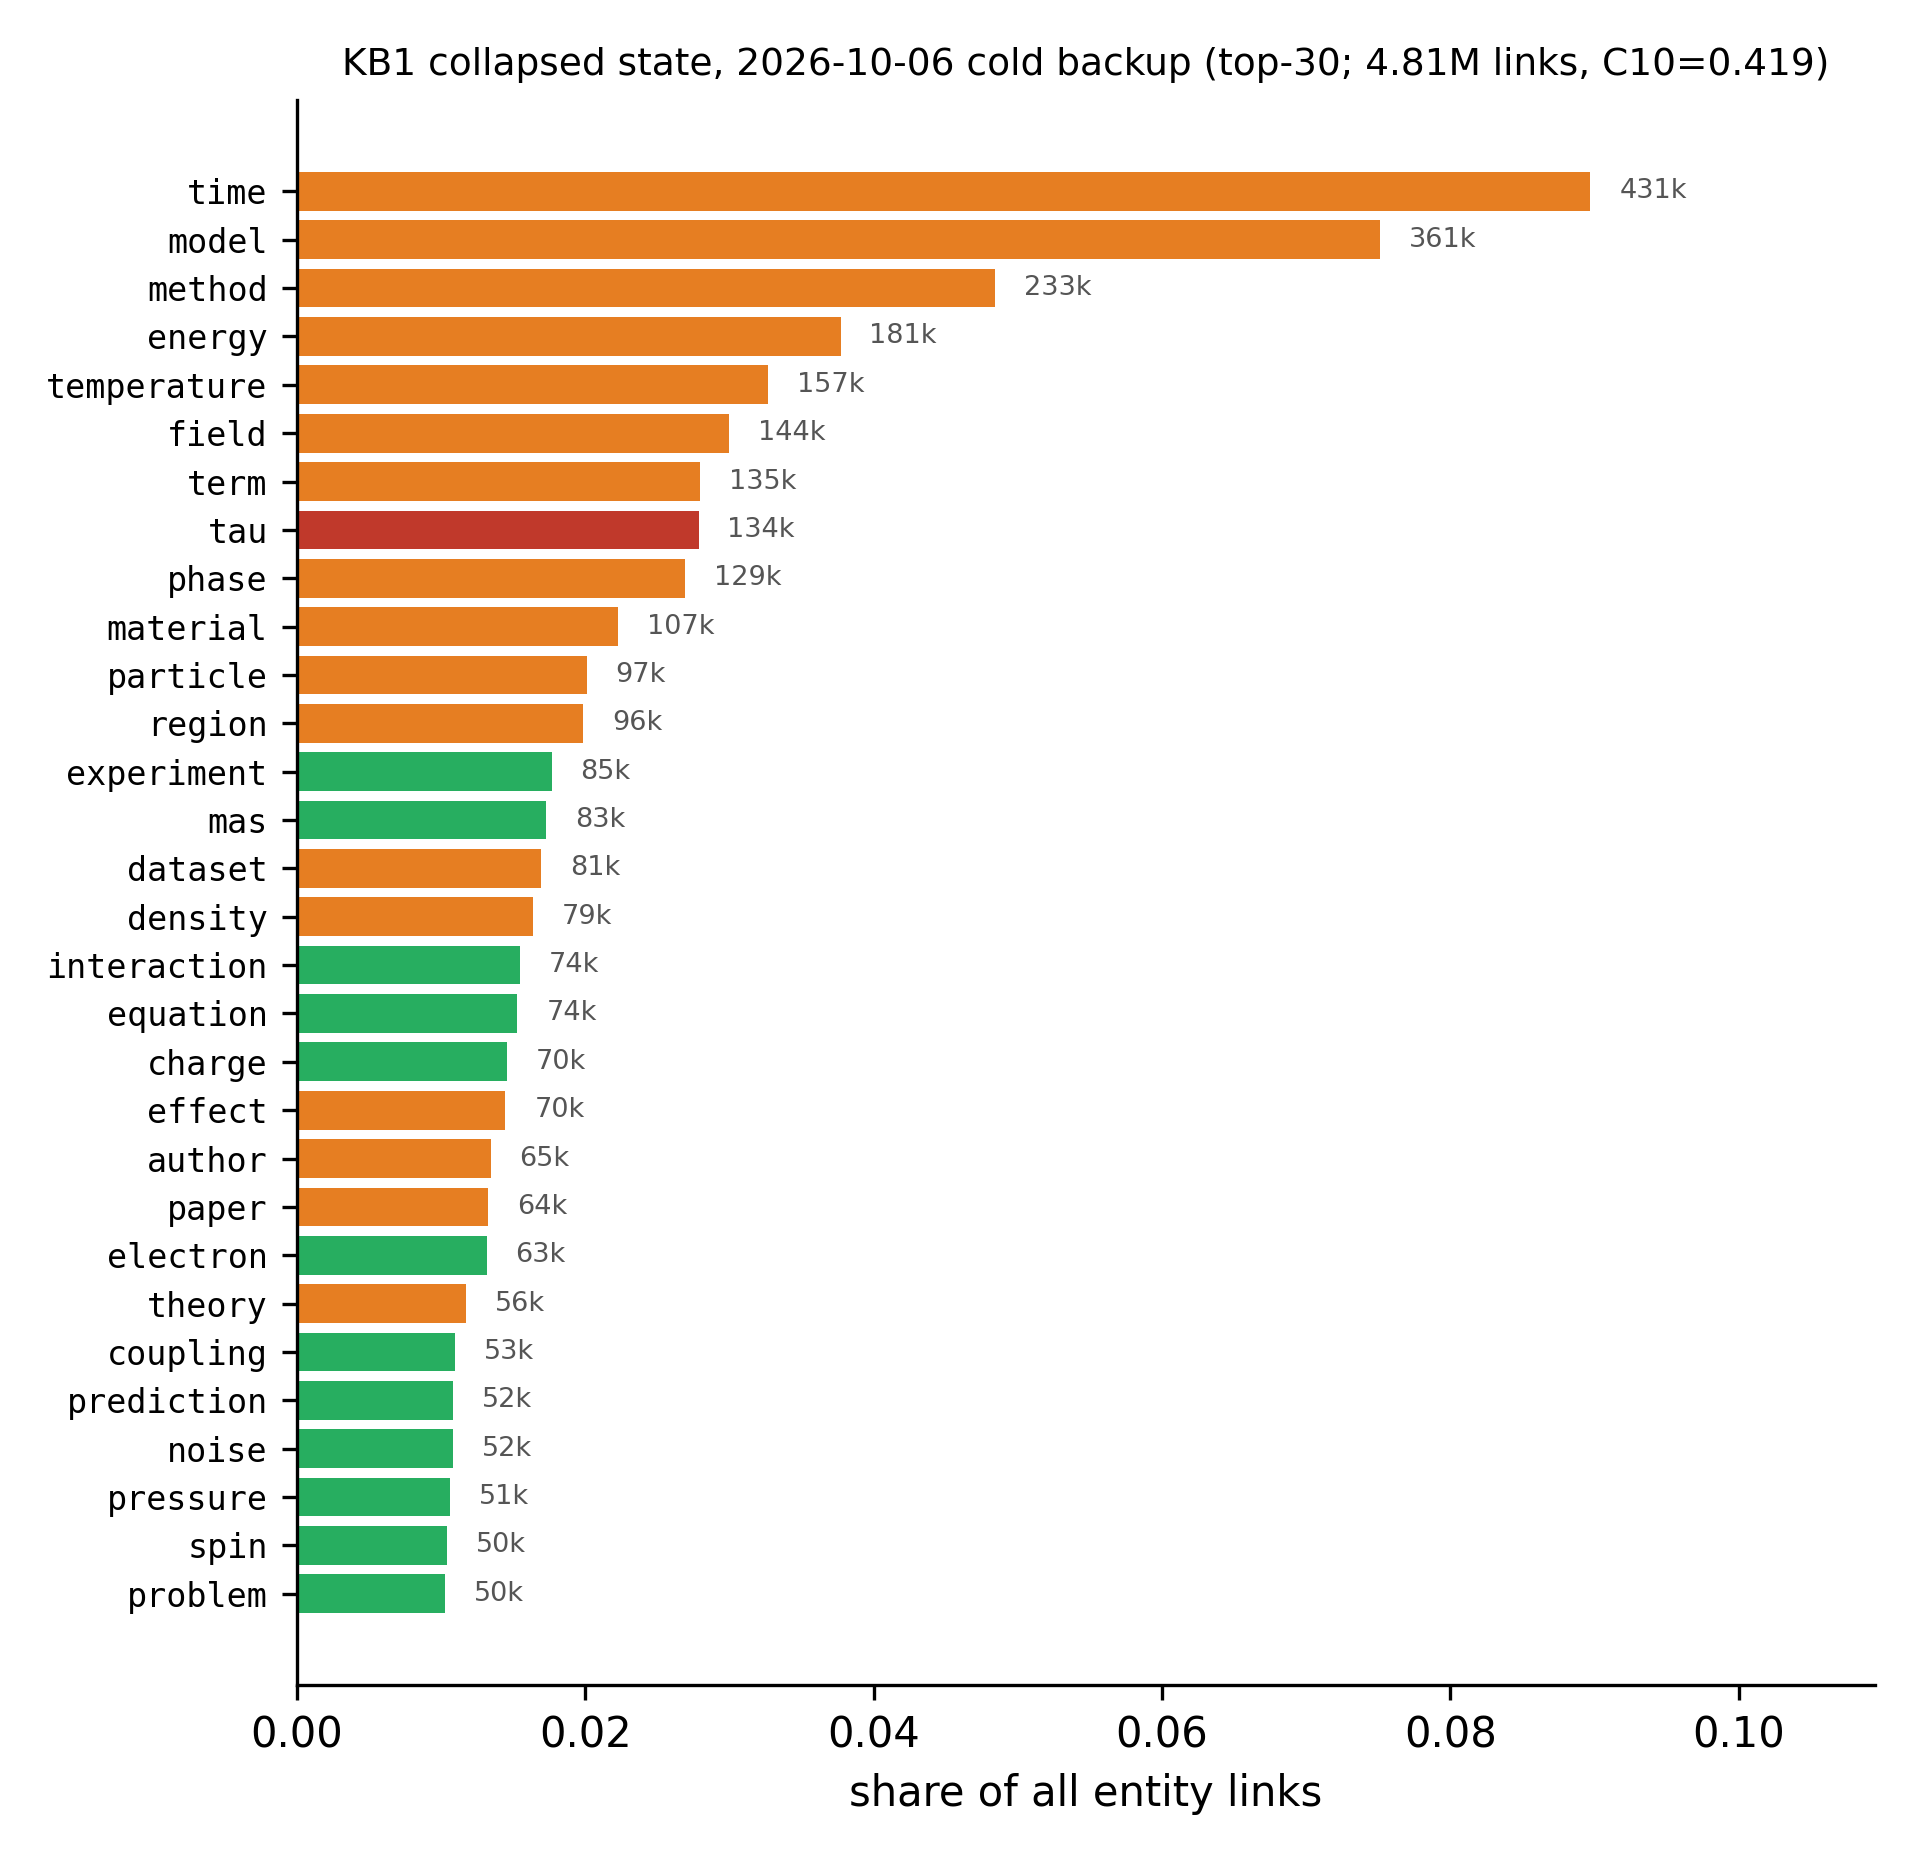
\includegraphics[width=0.98\columnwidth]{figs/fig_top_before.png}\\[1mm]
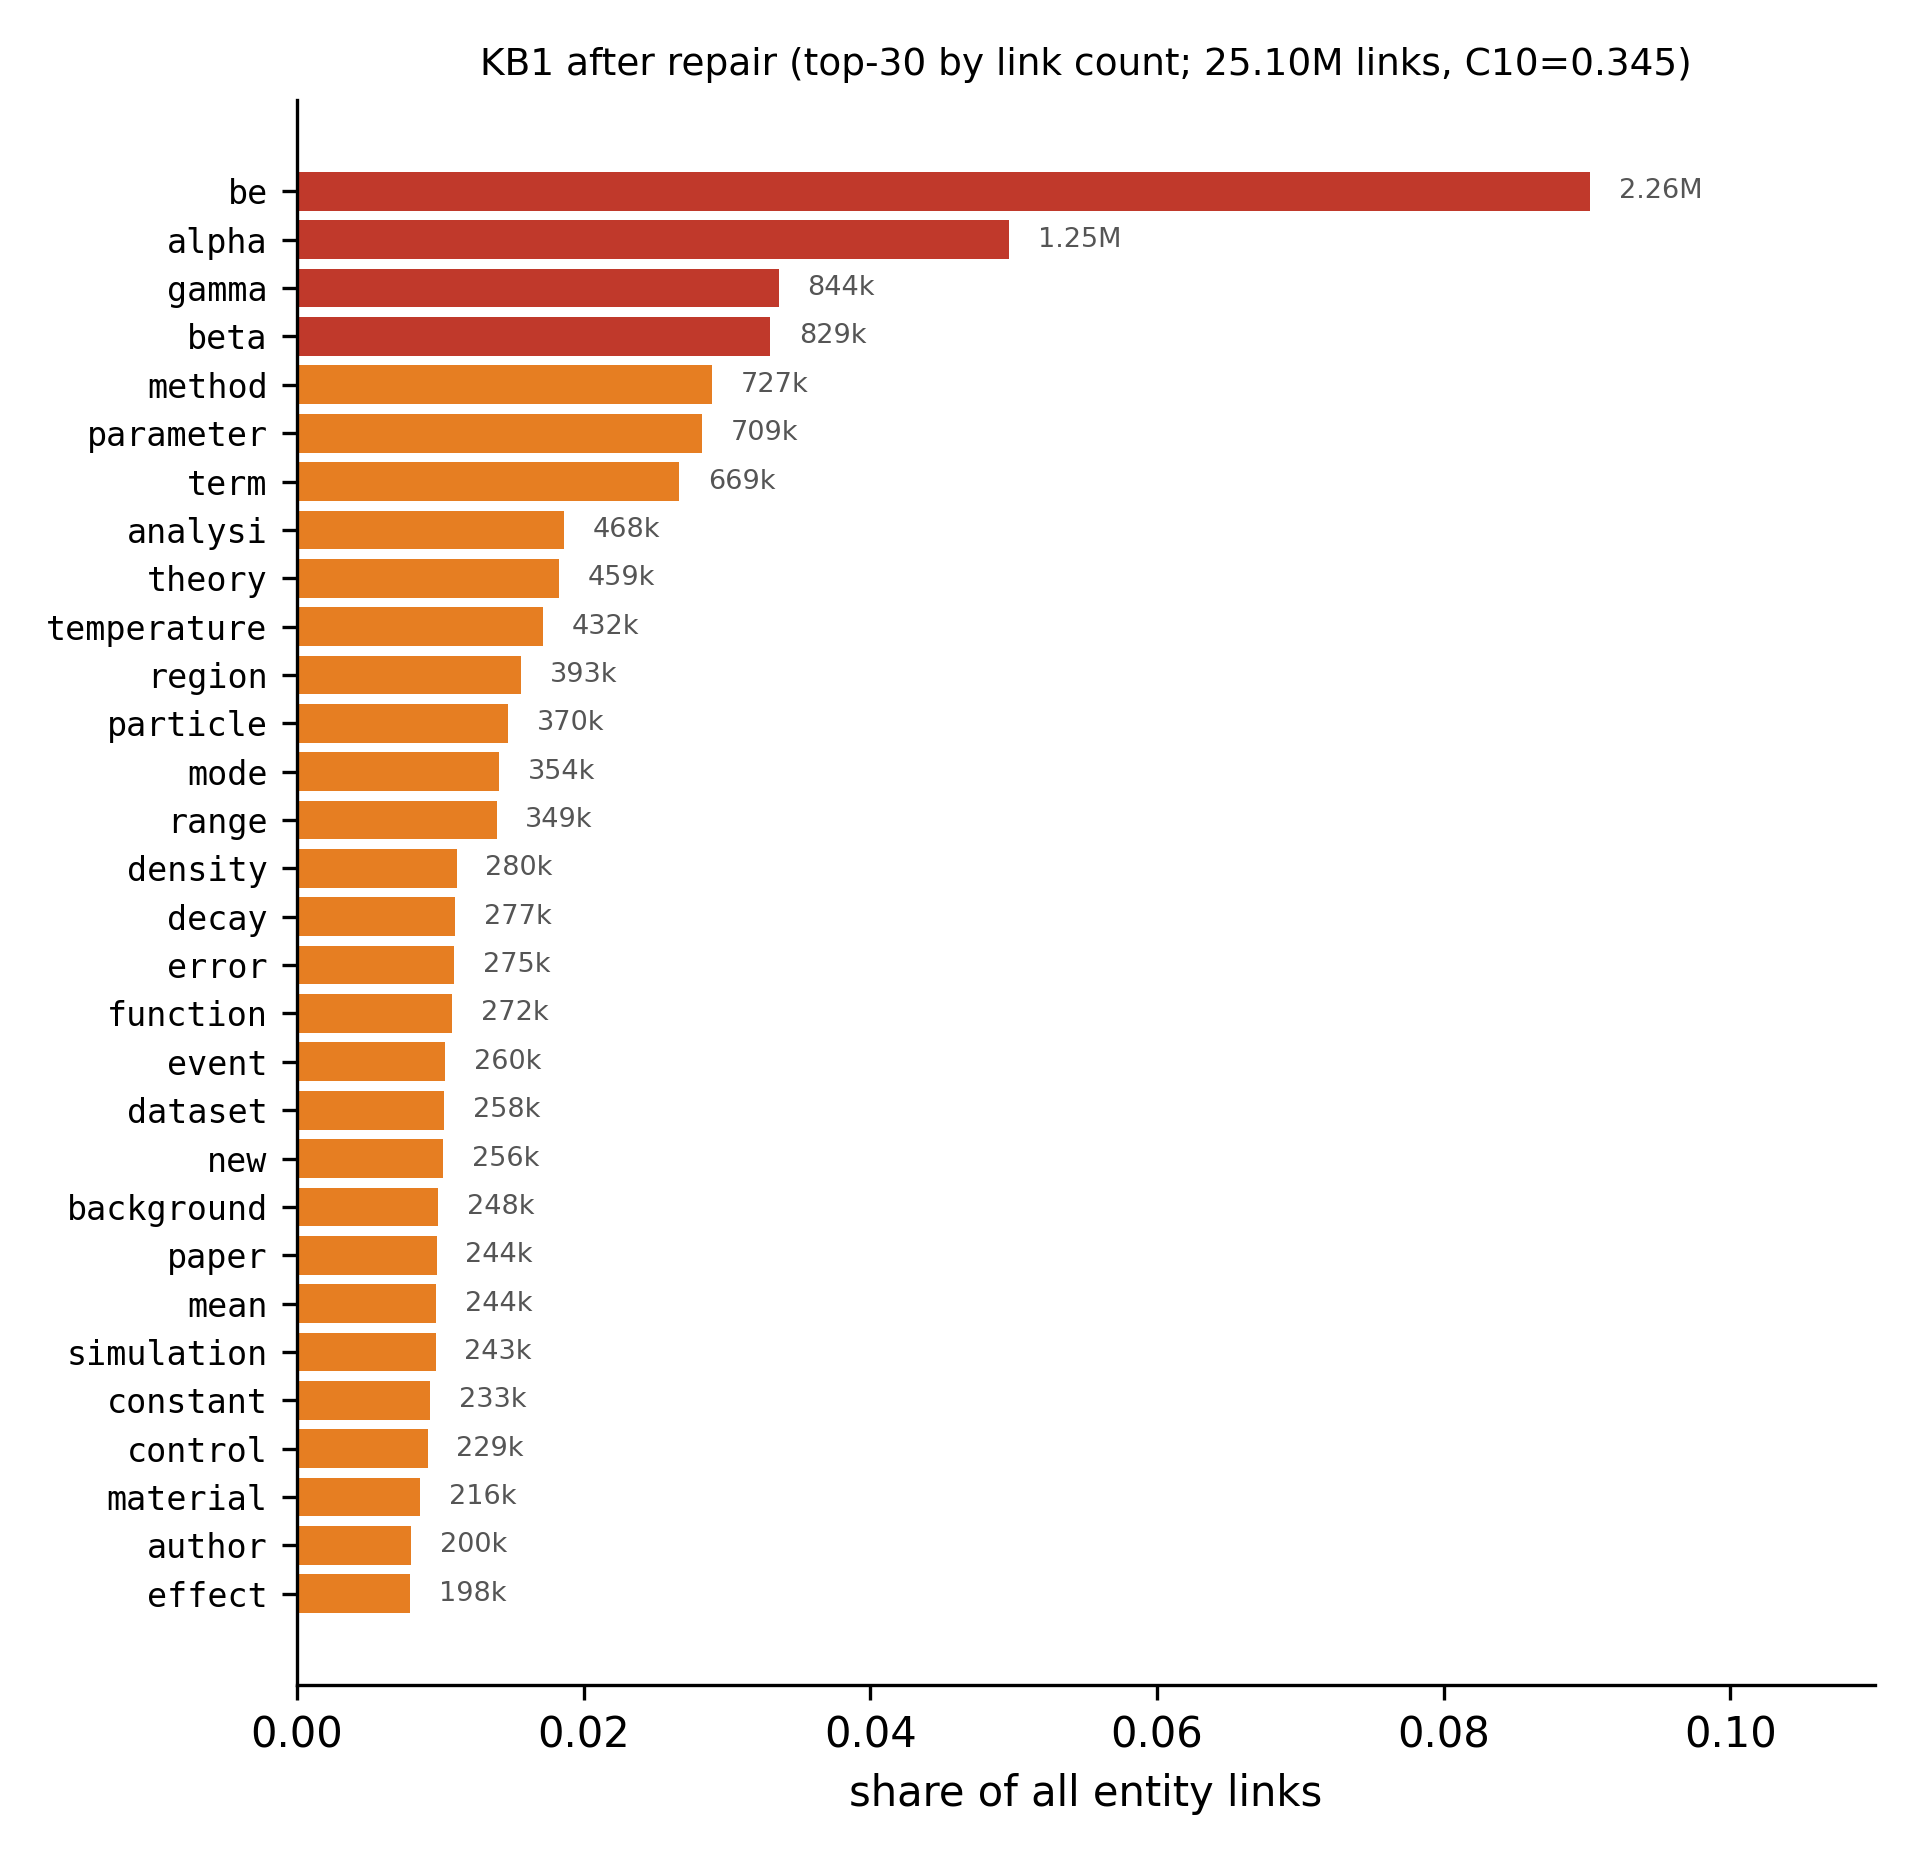
\includegraphics[width=0.98\columnwidth]{figs/fig_top_after.png}
\caption{Top-30 entities by link share, before (cold backup;
$C_{10}$=0.419) and after repair ($C_{10}$=0.345). Green = domain
terms, orange = generic words, red = short ambiguous symbols.}
\label{fig:topentities}
\end{figure}

\textbf{Retrieval: honest attribution.} Scoped coverage rose
$+$6.6/$+$7.3 points over the repair window, but three controls bound
the attribution: (a)~a single-variable channel ablation under the final
configuration is \emph{bitwise null} (removing all entity channels
changes no metric while halving latency; a forced-trigger check on the
natural-phrasing set shows the channels are alive --- 54/99 fired, and
killing them costs 20 losses / 0 wins); (b)~alias expansion, the one
entity-adjacent mechanism, is $+$1.5pt (ns) on the benchmarks at
2$\times$ latency; (c)~two same-configuration runs differ on exactly
one query (0.5pt noise floor). The trajectory is system-level; the
entity layer's retrieval-facing value runs through asset surfaces
(documented in the companion system manuscript~\cite{companion}), not
fusion votes.

\textbf{Link precision audit.} A seeded 100-link sample (span integrity
100/100) judged by strict rubric: precision \textbf{0.85} (Wilson CI
[0.77, 0.91]); domain stratum 25/25 (n=25 --- small); generic stratum
60/75. A second Qwen-series model re-adjudicated: 45/100 responses
unparseable (flash-tier), and on the 55-link parseable subset
agreement is 96.4\% (domain 14/14) --- a cross-model check on a subset,
not family-independent confirmation (Figure~\ref{fig:auditci}). Human
adjudication remains the decisive future control.

\begin{figure}[t]
\centering
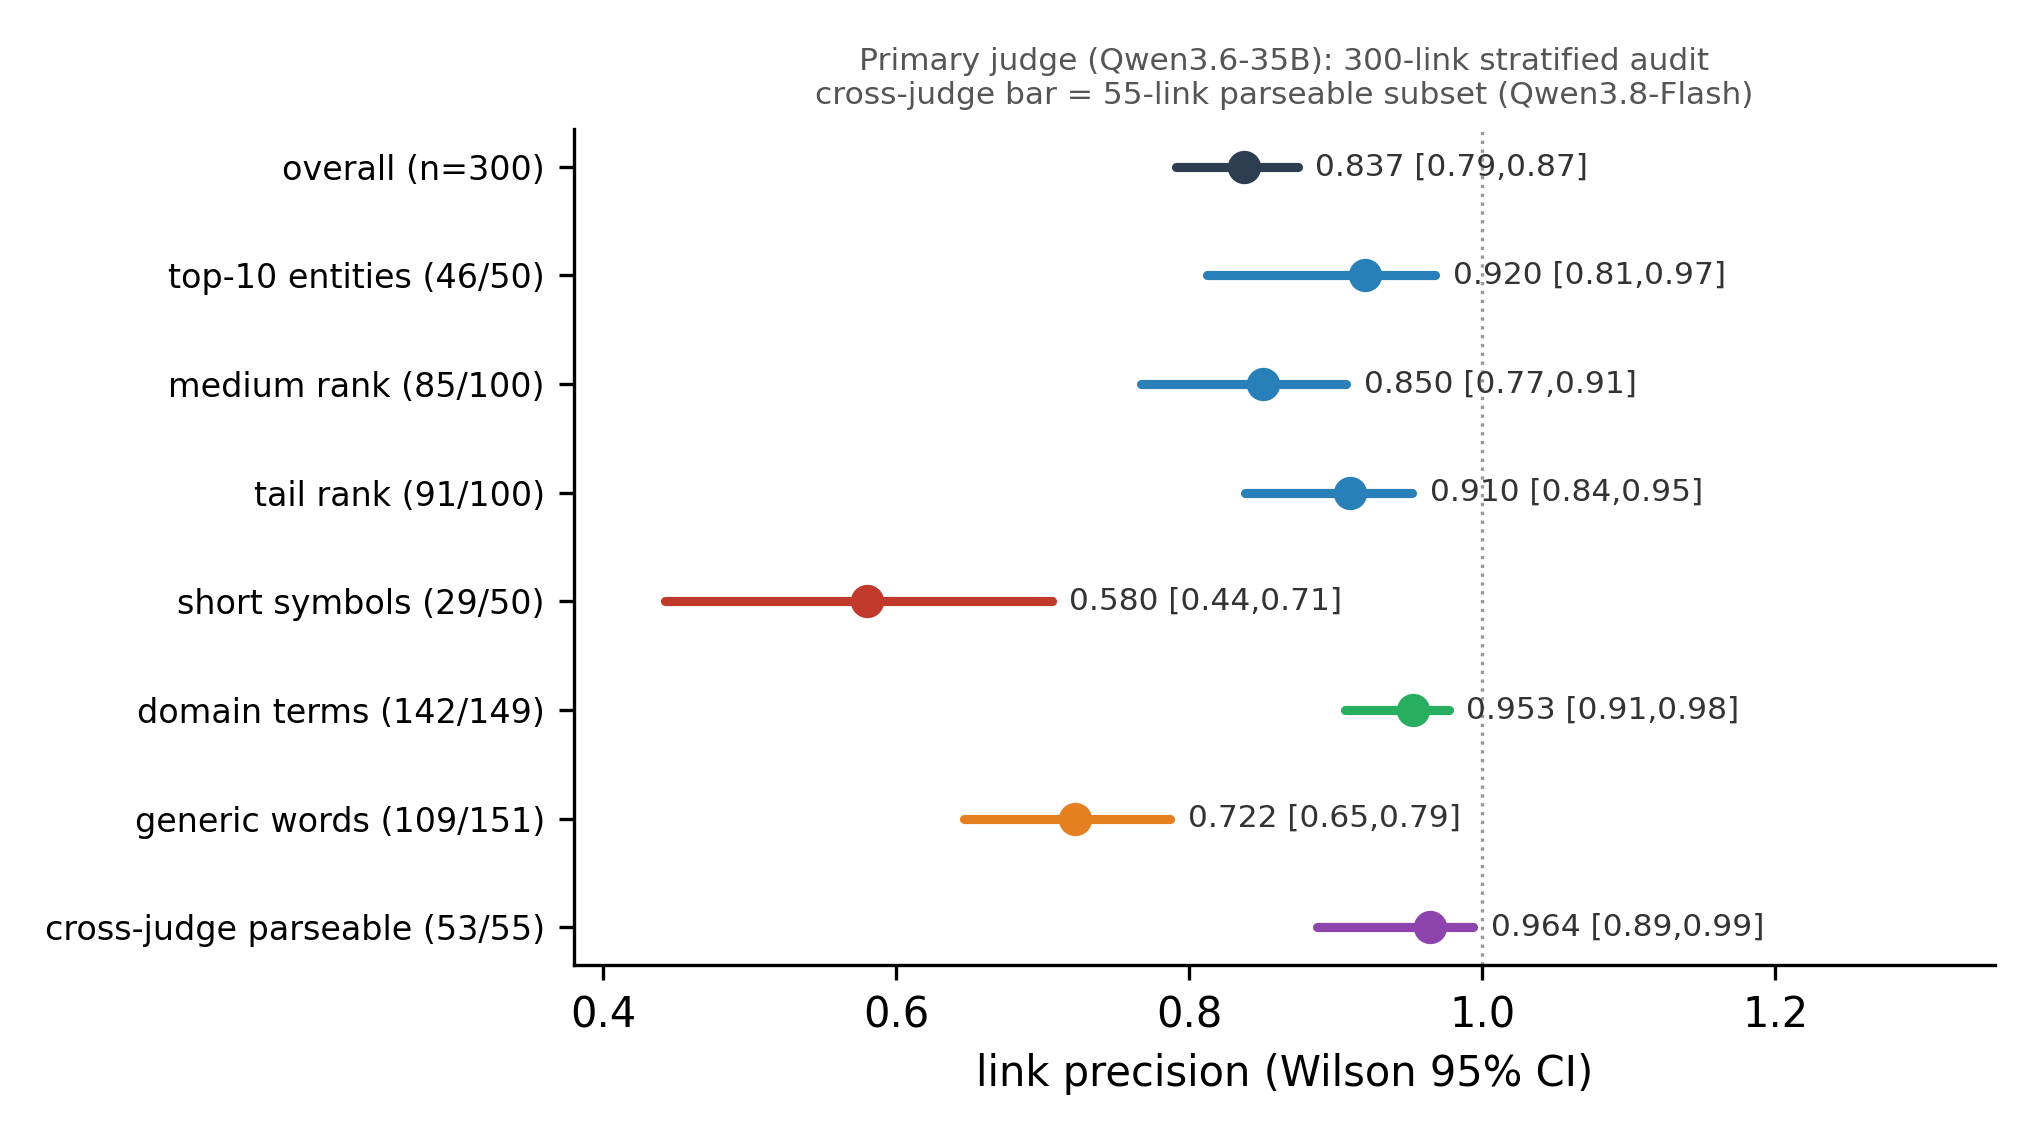
\includegraphics[width=0.98\columnwidth]{figs/fig_audit_ci.png}
\caption{Audit precision with Wilson 95\% CIs; cross-judge bars apply
to the 55-link parseable subset only.}
\label{fig:auditci}
\end{figure}

\subsection{The Lexicon Variable, Isolated}\label{sec:iso}

The repair bundled lexicon, teardown, and fleet changes; this experiment
isolates the lexicon alone: a semantic replica of the K1/K2 scan-and-link
semantics over a deterministic 2{,}000-chunk sample, with \emph{only the
dictionary swapped} --- v2.0 as committed at library creation (182 scan
terms), v2.5 mid-evolution (2{,}932), v2.1 the repair (3{,}733), plus
two v2.1 governance variants.

\begin{table}[t]
\centering
\caption{Isolated lexicon comparison (fixed code, fixed corpus).}
\label{tab:lexiso}
\small
\begin{tabularx}{\columnwidth}{@{}lXXXX@{}}
\toprule
Arm & Links & Ents & $C_{10}$ & Conc/doc \\
\midrule
v2.0 collapse-era & 2{,}720 & 77 & \textbf{0.557} & 1.8 \\
v2.5 mid & 4{,}472 & 266 & 0.339 & 2.4 \\
v2.1 repair & 9{,}456 & 493 & 0.316 & \textbf{3.7} \\
\;+case-sens.\ short & 8{,}328 & 468 & 0.290 & 3.4 \\
\;+stop-word block & 8{,}756 & 492 & \textbf{0.276} & 3.5 \\
\bottomrule
\end{tabularx}
\end{table}

Three findings (Table~\ref{tab:lexiso}). \textbf{(1)}~The collapse
signature is reproduced by the lexicon \emph{alone}: 77 entities,
$C_{10}$=0.557, 1.8 concepts/document --- same code, same corpus.
\textbf{(2)}~The repair effect is isolated: $\times$6.4 entities,
$\times$2.1 concepts/doc, generic-head mass 0.163$\to$0.062; the
production collapsed state (503 entities, $C_{10}$=0.419) sits between
the v2.0 and v2.5 counterfactuals, consistent with mid-enrichment
dictionary evolution. \textbf{(3)}~The \texttt{be} class is treatable
at known cost: case-sensitive short symbols remove the largest entity
(7.4\% of links; \texttt{be} leaves the top-5; $C_{10}\to$0.290) at a
fold-recall price (links $-$11.8\%, judged precision
0.95$\to$0.925); a stop-word block is gentler ($-$7.4\%, 0.276, 0.975).
Judged precision is near-tautological for dictionary self-matches, so
structural metrics lead. \emph{Provenance}: decomposing v2.1's link
mass by which committed lexicon first contained each term ---
v2.0-inherited 21.4\%, mid-evolution 15.3\%, \textbf{three-source-new
63.2\%} (296 of 493 entities); a true single-source regeneration
ablation remains future work.

\section{Monitors and Discussion}\label{sec:discussion}

\begin{figure}[t]
\centering
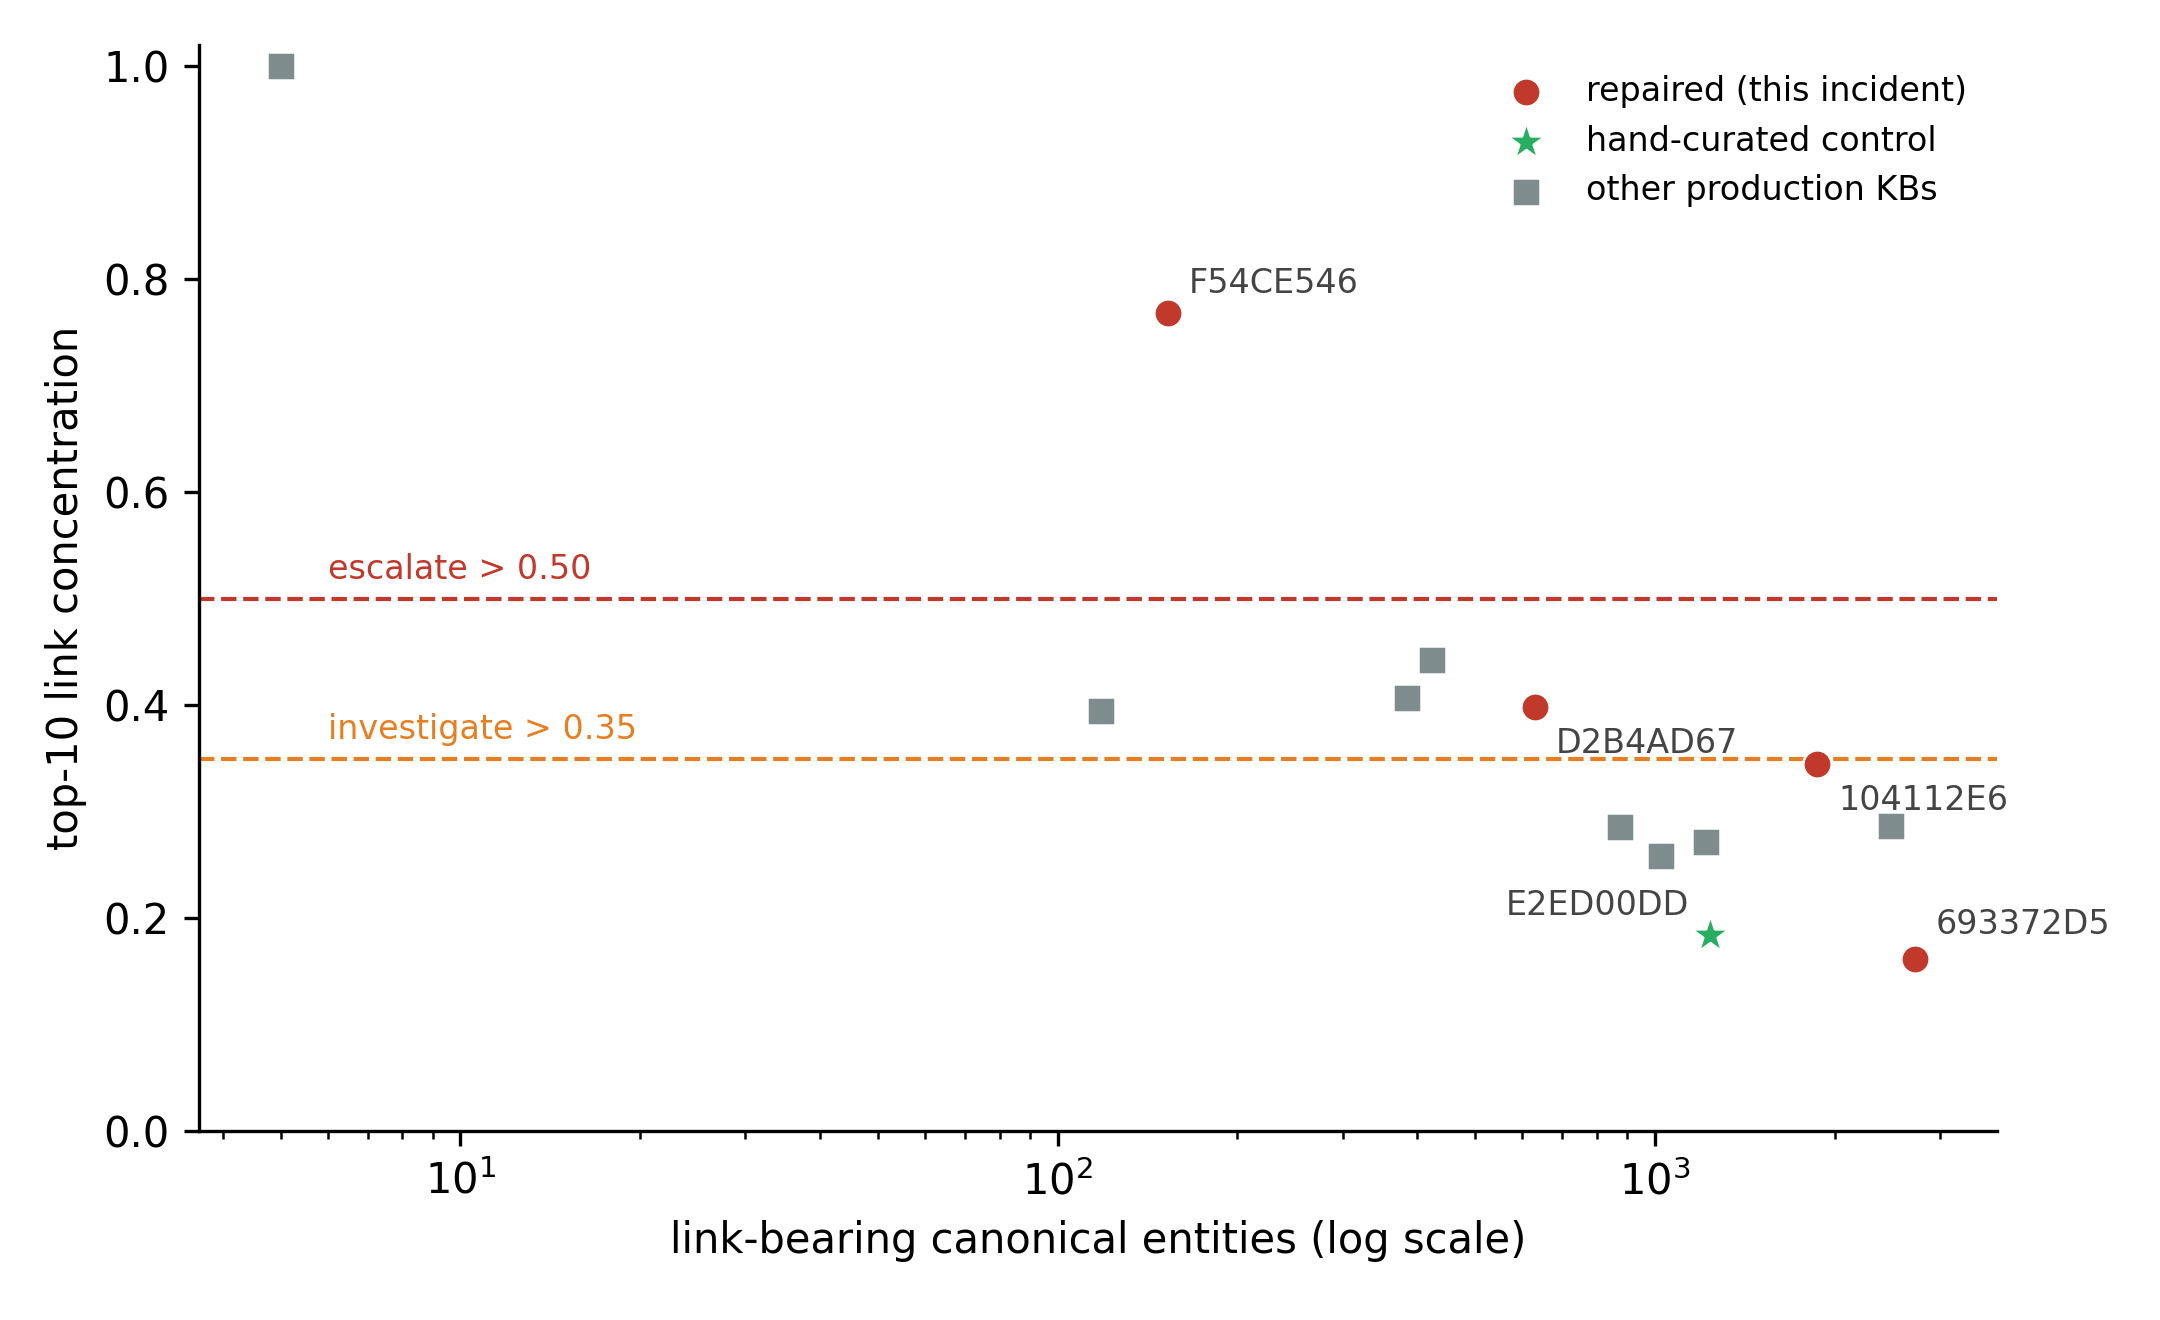
\includegraphics[width=0.92\columnwidth]{figs/fig_conc_scatter.png}
\caption{Top-10 link concentration vs.\ link-bearing entities across 13
production libraries; red = rebuilt in this incident, green star =
hand-curated reference. Bands are the proposed post-hoc thresholds.}
\label{fig:scatter}
\end{figure}

Four gold-free monitors, in the spirit of production data
validation~\cite{tdd}: \textbf{(a)~top-10 link concentration} (primary,
scale-invariant): across the 13 deployment libraries the metric spans
0.16--0.77; healthy/repaired large libraries run 0.16--0.19, the
rebuilt nuclear library 0.345, the two small treated libraries
\emph{currently} 0.398 and 0.768 (reported as measured --- the smallest
also shows the metric's Zipfian floor effect); collapsed state measured
0.419. Proposed bands ($>$0.35 investigate, $>$0.5 escalate) are
post-hoc on these 13 libraries --- a starting point, not a validated
norm; prospective validation is future work. \textbf{(b)~entity
cardinality ratio} (coarse secondary, gameable both ways).
\textbf{(c)~top-entity name audit} (five-minute quarterly control).
\textbf{(d)~target-table growth reconciliation} --- the B95 ghost-bucket
mechanism makes this mandatory wherever a bulk writer is guarded by
\texttt{INSERT IGNORE}. The small-library treatment doubles as
out-of-sample validation: cardinality normalized (870$\to$629,
209$\to$153) while concentration still flags both --- the two monitors
separate ``cardinality repaired'' from ``distribution still skewed.''

The incident is not an argument for LLM-everywhere: if extraction is a
scan, the dictionary \emph{is} the model and deserves a trained model's
evaluation discipline. Admission criteria (corpus presence) are
necessary but not sufficient; \emph{ranking} criteria (IDF-style
contrast, bilingual consistency, length/type priors) are the open
problem --- the generic tail is the standing evidence.

\section{Limitations}\label{sec:limitations}

(1)~The generic tail survives repair (9\% of links on ``be'').
(2)~Retrieval attribution is bounded, not eliminated: the full
lexicon$\times$configuration decomposition would require re-collapsing a
production library. (3)~Coverage: two libraries rebuilt, two smaller
treated; bilingual anomalies documented, not explained. (4)~Six
secondary incidents extended the repair; reported as findings.
(5)~Audit and cross-judge are model-assisted (same vendor family),
not human-adjudicated; a stratified human sample is the next
evaluation step. (6)~The isolated experiment uses a semantic-replica
scanner and committed-snapshot dictionaries, not independently
regenerated single-source lexicons.

\begin{acks}
Anonymous artifact: \url{https://github.com/simpleqt/knowledgenexus-artifact}
(evaluation drivers, audit adjudications, isolated-comparison results,
figures, and the companion system preprint).
\end{acks}

\bibliographystyle{ACM-Reference-Format}
\begin{thebibliography}{7}

\bibitem{cvalue} K.~Frantzi, S.~Ananiadou, H.~Mima. Automatic recognition
of multi-word terms: the C-value/NC-value method. \textit{Int. J. on
Digital Libraries} 3(2), 2000, 115--130.

\bibitem{nerSurvey} D.~Nadeau, S.~Sekine. A survey of named entity
recognition and classification. \textit{Lingvisticae Investigationes}
30(1), 2007, 3--26.

\bibitem{paulheim} H.~Paulheim. Knowledge graph refinement: A survey of
approaches and evaluation methods. \textit{Semantic Web} 8(3), 2017,
489--508.

\bibitem{tdd} N.~Polyzotis, S.~Roy, S.~E.~Whang, M.~Zinkevich. Data
validation for machine learning. \textit{Proc. MLSys}, 2019.

\bibitem{llmonto} A.~S.~Lippolis et al. Ontology generation using large
language models. arXiv:2503.05388, 2025.

\bibitem{iso1087} ISO 1087: Terminology work and terminology science ---
vocabulary. ISO, 2019.

\bibitem{companion} Anonymous. KnowledgeNexus: A traceable graph--vector
knowledge infrastructure and adaptive multi-channel retrieval for nuclear
science literature. Companion manuscript, under submission; preprint in
the artifact release.

\end{thebibliography}

\end{document}
